
\documentclass{beamer}
	\mode<presentation> {
	\usetheme{Hannover}
	% \setbeamertemplate{footline} % To remove the footer line in all slides uncomment this line
	\setbeamertemplate{footline}[page number] % To replace the footer line in all slides with a simple slide count uncomment this line
	\setbeamertemplate{navigation symbols}{} % To remove the navigation symbols from the bottom of all slides uncomment this line
	}

	\usepackage[utf8]{inputenc}

	\usepackage{graphicx}
	\graphicspath{{../Include/}}

	\usepackage{listings}
	\lstdefinestyle{mystyle}{
    breakatwhitespace=false,         
    breaklines=true,                 
    keepspaces=true,                 
    showspaces=false,                
    showstringspaces=false,
    showtabs=false
}
\lstset{style=mystyle}

	\usepackage{amsmath, mathrsfs}
	\usepackage{hyperref}
	\hypersetup{
	colorlinks=true,
	linkcolor=blue,
	filecolor=magenta,      
	urlcolor=blue,
	}
	
	\usepackage[backend=bibtex,style=numeric]{biblatex}
	\addbibresource{../Include/bibliografia.bib}
	\AtBeginBibliography{\scriptsize}





	\title[Anderson Acceleration]{Anderson Acceleration for Fixed-Point Iterations} 
		\subtitle {Project in Advanced Programming for Scientific Computing}
		\author[Martino Ischia]{Martino Ischia\\ \footnotesize{Supervisor: Prof. Formaggia}} 
		\institute[]
		{
		Politecnico di Milano
		}
		\date{Feb 19, 2020} 
		
		\begin{document}
			\begin{frame}
				\titlepage 
			\end{frame}
				
			\section{Introduction}
				\begin{frame}
					\frametitle{Context}
					\begin{itemize}
						\item Fixed-point iterations, looking for $x\in\mathbb{R}^n$ such that $x=g(x)$
						$$x_{k+1} = g(x_k)$$
						\item In the case where $g$ is nonlinear, \textbf{Newton method} typically shows quadratic convergence,
						whereas fixed-point form of the problem has typically linear convergence
						\item  Need for acceleration strategies
					\end{itemize}    
				\end{frame}
				
				
				\begin{frame}{Anderson Acceleration, \citeyear{Anderson} \cite{Anderson}}
					
					Given $x_0$ and $m \geq 1$\\
					Set $x_1 = g(x_0)$\\
					For $k = 1, 2, ...$\\
					\hspace*{16pt} Set $m_k = min\{m, k\}$\\
					\hspace*{20pt}Set $F_k = (f_{k-m_k}, ... , f_k)$, where $f_i = g(x_i)-x_{i}$\\
					\hspace*{20pt}Determine $\alpha^{(k)} = (\alpha^{(k)}
					_0 , ..., \alpha^{(k)}_{m_k} )^T$, subject to\\ \hspace*{20pt}$\sum^{m_k}_{i=0} {\alpha_i = 1}$, that solves
					$$\min_{\alpha=(\alpha_0,...,\alpha_{m_k} )^T} \|F_k \alpha\|_2$$\\
					\hspace*{20pt}Set $x_{k+1} =\sum^{m_k}
					_{i=0} {\alpha_i^{(k)} g(x_{k-m_{k}+i})}$    
				\end{frame}
				
				\begin{frame}{Anderson Acceleration}
					% In the linear case $g(x_k) = A x + b$,\\
						% since $\sum^{m_k}_{i=0} {\alpha_i = 1}$,
						% $$x_{k+1} =\sum^{m_k}
						% _{i=0} {\alpha_i^{(k)} g(x_{k-m_{k}+i})} = \sum^{m_k}
					% _{i=0} {g(\alpha_i^{(k)}x_{k-m_{k}+i})} $$
					\begin{itemize}
						\item A more compact update formula
						\begin{equation*}
							x_{k+1}=x_{k} + \beta f_k -(\mathscr{X}_k + \beta \mathscr{F}_k)(\mathscr{F}_k^T \mathscr{F}_k)^{-1}\mathscr{F}_k^T f_k
						\end{equation*}
						where
						$\mathscr{X}_k=[\Delta x_{k-m}...\Delta x_{k-1}]$ with $\Delta x_{i}=x_{i+1}-x_i$  
						$\mathscr{F}_k=[\Delta f_{k-m}...\Delta f_{k-1}]$ with $\Delta f_{i}=f_{i+1}-f_i$ and $f_i$ is still $g(x_i)-x_{i}$
						\item It is a particular case of multisecant updating method \cite{Fang}
						\item In the linear case, when $m = \infty$, GMRES solves the same least squares problem and $x_{k+1}^A = g(x_k^{GMRES})$
					\end{itemize}
				\end{frame}
					
				\section{C++ interface}
				
				\begin{frame}{Generic interface for fixed-point problems}
					\begin{itemize}
					\item	\href{file:///D:/VM/progetto/src/html/index.html}{Link} to the documentation.
					\item \texttt{DenseTraits} and \texttt{SparseTraits} based on the Eigen library version 3.
				\end{itemize}
				\end{frame}
				
				\begin{frame}[fragile]{The Iterator family}
					Constructor with universal references
						\begin{lstlisting}[basicstyle=\scriptsize, language=C++]
					template <class IterationFun>
					Iterator(IterationFun && IF, std::size_t dim):
					phi(std::forward<IterationFun>(IF)), dimension(dim){}
						\end{lstlisting}
						Call operator (virtual)
						\begin{lstlisting}[basicstyle=\scriptsize, language=C++]
					virtual Traits::Vector
					Iterator::operator()(const std::deque<Vector>& past){
					    assert (!past.empty());
					    return phi( past.back() );
					}
						\end{lstlisting}

				\end{frame}
				
				\begin{frame}{Anderson accelerator}
				\begin{itemize}
				\item \texttt{AndersonAccelerator} class stores
				$\mathscr{X}_k$ and $\mathscr{F}_k$ which are updated 
				only in the last column at each iteration. The \texttt{RotatingMatrix}
				template class does this efficiently.\\
				Let $P$ a permutation matrix (swapping columns of $A$ is $AP$)
				\begin{equation*}
					x_{k+1}=x_{k} + \beta f_k -(\mathscr{X}_k + \beta \mathscr{F}_k)P(P^T \mathscr{F}_k^T \mathscr{F}_k P)^{-1}P^T \mathscr{F}_k^T f_k
				\end{equation*}
				\begin{equation*}
					x_{k+1}=x_{k} + \beta f_k -(\mathscr{X}_k + \beta \mathscr{F}_k)P P^T (\mathscr{F}_k^T \mathscr{F}_k)^{-1} P P^T \mathscr{F}_k^T f_k
				\end{equation*}
				\item For solving the least-squares problem, the Householder rank-revealing
				QR decomposition with column-pivoting is used, that is a good compromise
				between numerical stability and efficiency.
				\end{itemize}
				\end{frame}
				
				
				
				\begin{frame}[fragile]{\texttt{FixedPointIterator} class}
						\begin{itemize}
						\item \verb|std::unique_ptr| to an \verb|Iterator| object
						\item \verb|options|, an options struct, controlling maximum iterations, tolerances and printing styles
								(stopping criterion is based on the distance of two iterates (stagnation))
						\item \verb|history|, an \verb|std::deque<Vector>| containing the history of the vector sequence
						\item \verb|iteration| number
						\item  \verb|compute()| and \verb|compute(const Vector&)|
						\item  methods to output a result (\verb|printResult| is one possibility)
						\end{itemize}	
				\end{frame}


				\section{Examples}
					
				\begin{frame}[fragile]{A first example}
				Usage:
				
				
				\begin{lstlisting}[basicstyle=\scriptsize, language=C++]
				FixedPointIterator FPI_1;
				FPI_1.setIterator( std::make_unique <Iterator> 
				                  (std::move(phi_1), dimension));
				FPI_1.compute(startingPoint_1);
				\end{lstlisting}
				
				
				on problem
				
				\begin{equation*}
							\left \lbrace 
									\begin{aligned}
									-\frac{1}{81}cos(x) + \frac{1}{9}y^2 + \frac{1}{3}z = x\\
									\frac{1}{3}x + \frac{1}{3}cos(z) = y\\
									-\frac{1}{9}cos(x) + \frac{1}{3}y + \frac{1}{6}sin(z) = z 
								\end{aligned}
								\right.
				\end{equation*}

				\end{frame}


				\begin{frame}{A first example}			
				\begin{figure}
				{\scriptsize
				% GNUPLOT: LaTeX picture with Postscript
\begingroup
  % Encoding inside the plot.  In the header of your document, this encoding
  % should to defined, e.g., by using
  % \usepackage[cp1252,<other encodings>]{inputenc}
  \inputencoding{cp1252}%
  \makeatletter
  \providecommand\color[2][]{%
    \GenericError{(gnuplot) \space\space\space\@spaces}{%
      Package color not loaded in conjunction with
      terminal option `colourtext'%
    }{See the gnuplot documentation for explanation.%
    }{Either use 'blacktext' in gnuplot or load the package
      color.sty in LaTeX.}%
    \renewcommand\color[2][]{}%
  }%
  \providecommand\includegraphics[2][]{%
    \GenericError{(gnuplot) \space\space\space\@spaces}{%
      Package graphicx or graphics not loaded%
    }{See the gnuplot documentation for explanation.%
    }{The gnuplot epslatex terminal needs graphicx.sty or graphics.sty.}%
    \renewcommand\includegraphics[2][]{}%
  }%
  \providecommand\rotatebox[2]{#2}%
  \@ifundefined{ifGPcolor}{%
    \newif\ifGPcolor
    \GPcolorfalse
  }{}%
  \@ifundefined{ifGPblacktext}{%
    \newif\ifGPblacktext
    \GPblacktexttrue
  }{}%
  % define a \g@addto@macro without @ in the name:
  \let\gplgaddtomacro\g@addto@macro
  % define empty templates for all commands taking text:
  \gdef\gplbacktext{}%
  \gdef\gplfronttext{}%
  \makeatother
  \ifGPblacktext
    % no textcolor at all
    \def\colorrgb#1{}%
    \def\colorgray#1{}%
  \else
    % gray or color?
    \ifGPcolor
      \def\colorrgb#1{\color[rgb]{#1}}%
      \def\colorgray#1{\color[gray]{#1}}%
      \expandafter\def\csname LTw\endcsname{\color{white}}%
      \expandafter\def\csname LTb\endcsname{\color{black}}%
      \expandafter\def\csname LTa\endcsname{\color{black}}%
      \expandafter\def\csname LT0\endcsname{\color[rgb]{1,0,0}}%
      \expandafter\def\csname LT1\endcsname{\color[rgb]{0,1,0}}%
      \expandafter\def\csname LT2\endcsname{\color[rgb]{0,0,1}}%
      \expandafter\def\csname LT3\endcsname{\color[rgb]{1,0,1}}%
      \expandafter\def\csname LT4\endcsname{\color[rgb]{0,1,1}}%
      \expandafter\def\csname LT5\endcsname{\color[rgb]{1,1,0}}%
      \expandafter\def\csname LT6\endcsname{\color[rgb]{0,0,0}}%
      \expandafter\def\csname LT7\endcsname{\color[rgb]{1,0.3,0}}%
      \expandafter\def\csname LT8\endcsname{\color[rgb]{0.5,0.5,0.5}}%
    \else
      % gray
      \def\colorrgb#1{\color{black}}%
      \def\colorgray#1{\color[gray]{#1}}%
      \expandafter\def\csname LTw\endcsname{\color{white}}%
      \expandafter\def\csname LTb\endcsname{\color{black}}%
      \expandafter\def\csname LTa\endcsname{\color{black}}%
      \expandafter\def\csname LT0\endcsname{\color{black}}%
      \expandafter\def\csname LT1\endcsname{\color{black}}%
      \expandafter\def\csname LT2\endcsname{\color{black}}%
      \expandafter\def\csname LT3\endcsname{\color{black}}%
      \expandafter\def\csname LT4\endcsname{\color{black}}%
      \expandafter\def\csname LT5\endcsname{\color{black}}%
      \expandafter\def\csname LT6\endcsname{\color{black}}%
      \expandafter\def\csname LT7\endcsname{\color{black}}%
      \expandafter\def\csname LT8\endcsname{\color{black}}%
    \fi
  \fi
    \setlength{\unitlength}{0.0500bp}%
    \ifx\gptboxheight\undefined%
      \newlength{\gptboxheight}%
      \newlength{\gptboxwidth}%
      \newsavebox{\gptboxtext}%
    \fi%
    \setlength{\fboxrule}{0.5pt}%
    \setlength{\fboxsep}{1pt}%
\begin{picture}(5668.00,2834.00)%
    \gplgaddtomacro\gplbacktext{%
      \csname LTb\endcsname%%
      \put(1220,806){\makebox(0,0)[r]{\strut{}$1\times10^{-10}$}}%
      \put(1220,1138){\makebox(0,0)[r]{\strut{}$1\times10^{-8}$}}%
      \put(1220,1470){\makebox(0,0)[r]{\strut{}$1\times10^{-6}$}}%
      \put(1220,1803){\makebox(0,0)[r]{\strut{}$0.0001$}}%
      \put(1220,2135){\makebox(0,0)[r]{\strut{}$0.01$}}%
      \put(1220,2467){\makebox(0,0)[r]{\strut{}$1$}}%
      \put(1340,440){\makebox(0,0){\strut{}$0$}}%
      \put(2001,440){\makebox(0,0){\strut{}$5$}}%
      \put(2662,440){\makebox(0,0){\strut{}$10$}}%
      \put(3324,440){\makebox(0,0){\strut{}$15$}}%
      \put(3985,440){\makebox(0,0){\strut{}$20$}}%
      \put(4646,440){\makebox(0,0){\strut{}$25$}}%
      \put(5307,440){\makebox(0,0){\strut{}$30$}}%
    }%
    \gplgaddtomacro\gplfronttext{%
      \csname LTb\endcsname%%
      \put(190,1636){\rotatebox{-270}{\makebox(0,0){\strut{}Residual}}}%
      \put(3323,140){\makebox(0,0){\strut{}Iteration \#}}%
      \csname LTb\endcsname%%
      \put(4404,2470){\makebox(0,0)[r]{\strut{}Fixed-point iterations}}%
      \csname LTb\endcsname%%
      \put(4404,2270){\makebox(0,0)[r]{\strut{}Anderson algorithm}}%
    }%
    \gplbacktext
    \put(0,0){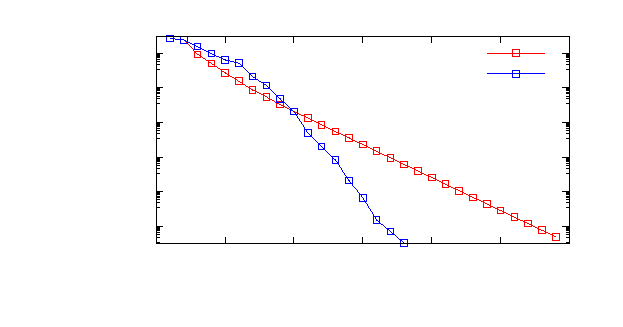
\includegraphics{./Include/simple_example_residuals}}%
    \gplfronttext
  \end{picture}%
\endgroup
}
				\centering
				\caption{\textit{Residual vs Interation number for the nonlinear 3D problem.
				Parameters of Anderson algorithm are $\beta=1$ $m=5$.}}
				\end{figure}
			
				\end{frame}

				\begin{frame}{Linear FEM example}
				Heat equation matrix:
				\begin{equation*}
				A=\left[
				\begin{array}{llllll}
				2+h^2a & -1 & 0 &\ldots&\ldots& 0\\
				-1 & 2+h^2a & -1 &\ldots&\ldots& 0\\
				 &   & \ldots &\ldots& & \\
				0  & \ldots & \ldots &-1 &2+h^2a& -1\\
				0  & \ldots & \ldots &\ldots&-1& 1\\
				\end{array}
				\right]
				\end{equation*}

				Matrix $A$ is symmetric positive definite: the
				Gauss-Seidel iterative scheme will converge to the solution.
				\end{frame}
				
				\begin{frame}{Accelerating Gauss-Seidel}
			\begin{figure}
			{\scriptsize
			% GNUPLOT: LaTeX picture with Postscript
\begingroup
  % Encoding inside the plot.  In the header of your document, this encoding
  % should to defined, e.g., by using
  % \usepackage[cp1252,<other encodings>]{inputenc}
  \inputencoding{cp1252}%
  \makeatletter
  \providecommand\color[2][]{%
    \GenericError{(gnuplot) \space\space\space\@spaces}{%
      Package color not loaded in conjunction with
      terminal option `colourtext'%
    }{See the gnuplot documentation for explanation.%
    }{Either use 'blacktext' in gnuplot or load the package
      color.sty in LaTeX.}%
    \renewcommand\color[2][]{}%
  }%
  \providecommand\includegraphics[2][]{%
    \GenericError{(gnuplot) \space\space\space\@spaces}{%
      Package graphicx or graphics not loaded%
    }{See the gnuplot documentation for explanation.%
    }{The gnuplot epslatex terminal needs graphicx.sty or graphics.sty.}%
    \renewcommand\includegraphics[2][]{}%
  }%
  \providecommand\rotatebox[2]{#2}%
  \@ifundefined{ifGPcolor}{%
    \newif\ifGPcolor
    \GPcolorfalse
  }{}%
  \@ifundefined{ifGPblacktext}{%
    \newif\ifGPblacktext
    \GPblacktexttrue
  }{}%
  % define a \g@addto@macro without @ in the name:
  \let\gplgaddtomacro\g@addto@macro
  % define empty templates for all commands taking text:
  \gdef\gplbacktext{}%
  \gdef\gplfronttext{}%
  \makeatother
  \ifGPblacktext
    % no textcolor at all
    \def\colorrgb#1{}%
    \def\colorgray#1{}%
  \else
    % gray or color?
    \ifGPcolor
      \def\colorrgb#1{\color[rgb]{#1}}%
      \def\colorgray#1{\color[gray]{#1}}%
      \expandafter\def\csname LTw\endcsname{\color{white}}%
      \expandafter\def\csname LTb\endcsname{\color{black}}%
      \expandafter\def\csname LTa\endcsname{\color{black}}%
      \expandafter\def\csname LT0\endcsname{\color[rgb]{1,0,0}}%
      \expandafter\def\csname LT1\endcsname{\color[rgb]{0,1,0}}%
      \expandafter\def\csname LT2\endcsname{\color[rgb]{0,0,1}}%
      \expandafter\def\csname LT3\endcsname{\color[rgb]{1,0,1}}%
      \expandafter\def\csname LT4\endcsname{\color[rgb]{0,1,1}}%
      \expandafter\def\csname LT5\endcsname{\color[rgb]{1,1,0}}%
      \expandafter\def\csname LT6\endcsname{\color[rgb]{0,0,0}}%
      \expandafter\def\csname LT7\endcsname{\color[rgb]{1,0.3,0}}%
      \expandafter\def\csname LT8\endcsname{\color[rgb]{0.5,0.5,0.5}}%
    \else
      % gray
      \def\colorrgb#1{\color{black}}%
      \def\colorgray#1{\color[gray]{#1}}%
      \expandafter\def\csname LTw\endcsname{\color{white}}%
      \expandafter\def\csname LTb\endcsname{\color{black}}%
      \expandafter\def\csname LTa\endcsname{\color{black}}%
      \expandafter\def\csname LT0\endcsname{\color{black}}%
      \expandafter\def\csname LT1\endcsname{\color{black}}%
      \expandafter\def\csname LT2\endcsname{\color{black}}%
      \expandafter\def\csname LT3\endcsname{\color{black}}%
      \expandafter\def\csname LT4\endcsname{\color{black}}%
      \expandafter\def\csname LT5\endcsname{\color{black}}%
      \expandafter\def\csname LT6\endcsname{\color{black}}%
      \expandafter\def\csname LT7\endcsname{\color{black}}%
      \expandafter\def\csname LT8\endcsname{\color{black}}%
    \fi
  \fi
    \setlength{\unitlength}{0.0500bp}%
    \ifx\gptboxheight\undefined%
      \newlength{\gptboxheight}%
      \newlength{\gptboxwidth}%
      \newsavebox{\gptboxtext}%
    \fi%
    \setlength{\fboxrule}{0.5pt}%
    \setlength{\fboxsep}{1pt}%
\begin{picture}(5668.00,2834.00)%
    \gplgaddtomacro\gplbacktext{%
      \csname LTb\endcsname%%
      \put(1342,704){\makebox(0,0)[r]{\strut{}$1\times10^{-12}$}}%
      \put(1342,1051){\makebox(0,0)[r]{\strut{}$1\times10^{-10}$}}%
      \put(1342,1398){\makebox(0,0)[r]{\strut{}$1\times10^{-8}$}}%
      \put(1342,1745){\makebox(0,0)[r]{\strut{}$1\times10^{-6}$}}%
      \put(1342,2092){\makebox(0,0)[r]{\strut{}$0.0001$}}%
      \put(1342,2439){\makebox(0,0)[r]{\strut{}$0.01$}}%
      \put(1474,484){\makebox(0,0){\strut{}$0$}}%
      \put(1949,484){\makebox(0,0){\strut{}$10$}}%
      \put(2423,484){\makebox(0,0){\strut{}$20$}}%
      \put(2898,484){\makebox(0,0){\strut{}$30$}}%
      \put(3373,484){\makebox(0,0){\strut{}$40$}}%
      \put(3847,484){\makebox(0,0){\strut{}$50$}}%
      \put(4322,484){\makebox(0,0){\strut{}$60$}}%
      \put(4796,484){\makebox(0,0){\strut{}$70$}}%
      \put(5271,484){\makebox(0,0){\strut{}$80$}}%
    }%
    \gplgaddtomacro\gplfronttext{%
      \csname LTb\endcsname%%
      \put(209,1658){\rotatebox{-270}{\makebox(0,0){\strut{}Residual}}}%
      \put(3372,154){\makebox(0,0){\strut{}Iteration \#}}%
      \csname LTb\endcsname%%
      \put(2461,1097){\makebox(0,0)[l]{\strut{}Gauss-Seidel iterations}}%
      \csname LTb\endcsname%%
      \put(2461,877){\makebox(0,0)[l]{\strut{}Anderson algorithm}}%
    }%
    \gplbacktext
    \put(0,0){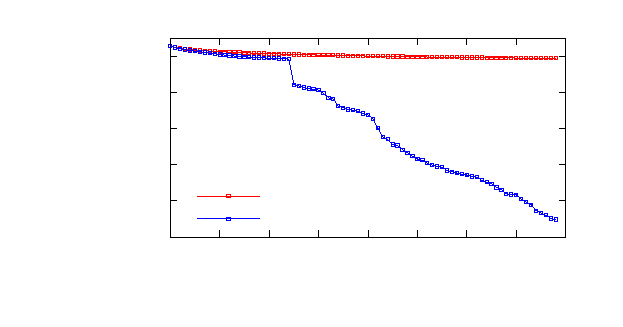
\includegraphics{gauss}}%
    \gplfronttext
  \end{picture}%
\endgroup
}
			\centering
			\caption{\textit{Gauss-Seidel problem with mesh $size=25$}}
			\end{figure}
			\end{frame}
			
			
			\begin{frame}[fragile]{Parameters testing}
			\begin{figure}
			{\scriptsize
			\resizebox{\textwidth}{!}{% GNUPLOT: LaTeX picture with Postscript
\begingroup
  % Encoding inside the plot.  In the header of your document, this encoding
  % should to defined, e.g., by using
  % \usepackage[cp1252,<other encodings>]{inputenc}
  \inputencoding{cp1252}%
  \makeatletter
  \providecommand\color[2][]{%
    \GenericError{(gnuplot) \space\space\space\@spaces}{%
      Package color not loaded in conjunction with
      terminal option `colourtext'%
    }{See the gnuplot documentation for explanation.%
    }{Either use 'blacktext' in gnuplot or load the package
      color.sty in LaTeX.}%
    \renewcommand\color[2][]{}%
  }%
  \providecommand\includegraphics[2][]{%
    \GenericError{(gnuplot) \space\space\space\@spaces}{%
      Package graphicx or graphics not loaded%
    }{See the gnuplot documentation for explanation.%
    }{The gnuplot epslatex terminal needs graphicx.sty or graphics.sty.}%
    \renewcommand\includegraphics[2][]{}%
  }%
  \providecommand\rotatebox[2]{#2}%
  \@ifundefined{ifGPcolor}{%
    \newif\ifGPcolor
    \GPcolortrue
  }{}%
  \@ifundefined{ifGPblacktext}{%
    \newif\ifGPblacktext
    \GPblacktexttrue
  }{}%
  % define a \g@addto@macro without @ in the name:
  \let\gplgaddtomacro\g@addto@macro
  % define empty templates for all commands taking text:
  \gdef\gplbacktext{}%
  \gdef\gplfronttext{}%
  \makeatother
  \ifGPblacktext
    % no textcolor at all
    \def\colorrgb#1{}%
    \def\colorgray#1{}%
  \else
    % gray or color?
    \ifGPcolor
      \def\colorrgb#1{\color[rgb]{#1}}%
      \def\colorgray#1{\color[gray]{#1}}%
      \expandafter\def\csname LTw\endcsname{\color{white}}%
      \expandafter\def\csname LTb\endcsname{\color{black}}%
      \expandafter\def\csname LTa\endcsname{\color{black}}%
      \expandafter\def\csname LT0\endcsname{\color[rgb]{1,0,0}}%
      \expandafter\def\csname LT1\endcsname{\color[rgb]{0,1,0}}%
      \expandafter\def\csname LT2\endcsname{\color[rgb]{0,0,1}}%
      \expandafter\def\csname LT3\endcsname{\color[rgb]{1,0,1}}%
      \expandafter\def\csname LT4\endcsname{\color[rgb]{0,1,1}}%
      \expandafter\def\csname LT5\endcsname{\color[rgb]{1,1,0}}%
      \expandafter\def\csname LT6\endcsname{\color[rgb]{0,0,0}}%
      \expandafter\def\csname LT7\endcsname{\color[rgb]{1,0.3,0}}%
      \expandafter\def\csname LT8\endcsname{\color[rgb]{0.5,0.5,0.5}}%
    \else
      % gray
      \def\colorrgb#1{\color{black}}%
      \def\colorgray#1{\color[gray]{#1}}%
      \expandafter\def\csname LTw\endcsname{\color{white}}%
      \expandafter\def\csname LTb\endcsname{\color{black}}%
      \expandafter\def\csname LTa\endcsname{\color{black}}%
      \expandafter\def\csname LT0\endcsname{\color{black}}%
      \expandafter\def\csname LT1\endcsname{\color{black}}%
      \expandafter\def\csname LT2\endcsname{\color{black}}%
      \expandafter\def\csname LT3\endcsname{\color{black}}%
      \expandafter\def\csname LT4\endcsname{\color{black}}%
      \expandafter\def\csname LT5\endcsname{\color{black}}%
      \expandafter\def\csname LT6\endcsname{\color{black}}%
      \expandafter\def\csname LT7\endcsname{\color{black}}%
      \expandafter\def\csname LT8\endcsname{\color{black}}%
    \fi
  \fi
    \setlength{\unitlength}{0.0500bp}%
    \ifx\gptboxheight\undefined%
      \newlength{\gptboxheight}%
      \newlength{\gptboxwidth}%
      \newsavebox{\gptboxtext}%
    \fi%
    \setlength{\fboxrule}{0.5pt}%
    \setlength{\fboxsep}{1pt}%
\begin{picture}(9070.00,4534.00)%
    \gplgaddtomacro\gplbacktext{%
      \csname LTb\endcsname%%
      \put(682,930){\makebox(0,0)[r]{\strut{}2}}%
      \put(682,1381){\makebox(0,0)[r]{\strut{}4}}%
      \put(682,1832){\makebox(0,0)[r]{\strut{}6}}%
      \put(682,2283){\makebox(0,0)[r]{\strut{}8}}%
      \put(682,2734){\makebox(0,0)[r]{\strut{}10}}%
      \put(682,3185){\makebox(0,0)[r]{\strut{}15}}%
      \put(682,3636){\makebox(0,0)[r]{\strut{}20}}%
      \put(682,4087){\makebox(0,0)[r]{\strut{}25}}%
      \put(1052,484){\makebox(0,0){\strut{}1e-06}}%
      \put(1528,484){\makebox(0,0){\strut{}1e-05}}%
      \put(2004,484){\makebox(0,0){\strut{}0.0001}}%
      \put(2480,484){\makebox(0,0){\strut{}0.001}}%
      \put(2956,484){\makebox(0,0){\strut{}0.01}}%
      \put(3432,484){\makebox(0,0){\strut{}0.1}}%
      \put(3908,484){\makebox(0,0){\strut{}0.5}}%
      \put(4383,484){\makebox(0,0){\strut{}1}}%
      \put(4859,484){\makebox(0,0){\strut{}2}}%
      \put(5335,484){\makebox(0,0){\strut{}5}}%
      \put(5811,484){\makebox(0,0){\strut{}10}}%
      \put(6287,484){\makebox(0,0){\strut{}50}}%
      \put(6763,484){\makebox(0,0){\strut{}100}}%
      \put(7239,484){\makebox(0,0){\strut{}1000}}%
    }%
    \gplgaddtomacro\gplfronttext{%
      \csname LTb\endcsname%%
      \put(209,2508){\rotatebox{-270}{\makebox(0,0){\strut{}$m$ (memory)}}}%
      \put(4145,154){\makebox(0,0){\strut{}$\beta$ (relaxation)}}%
      \csname LTb\endcsname%%
      \put(8109,1190){\makebox(0,0)[l]{\strut{}$0.001$}}%
      \put(8109,2657){\makebox(0,0)[l]{\strut{}$0.01$}}%
      \put(8109,4125){\makebox(0,0)[l]{\strut{}$0.1$}}%
      \put(8835,2508){\rotatebox{-270}{\makebox(0,0){\strut{}Time taken ($s$)}}}%
    }%
    \gplbacktext
    \put(0,0){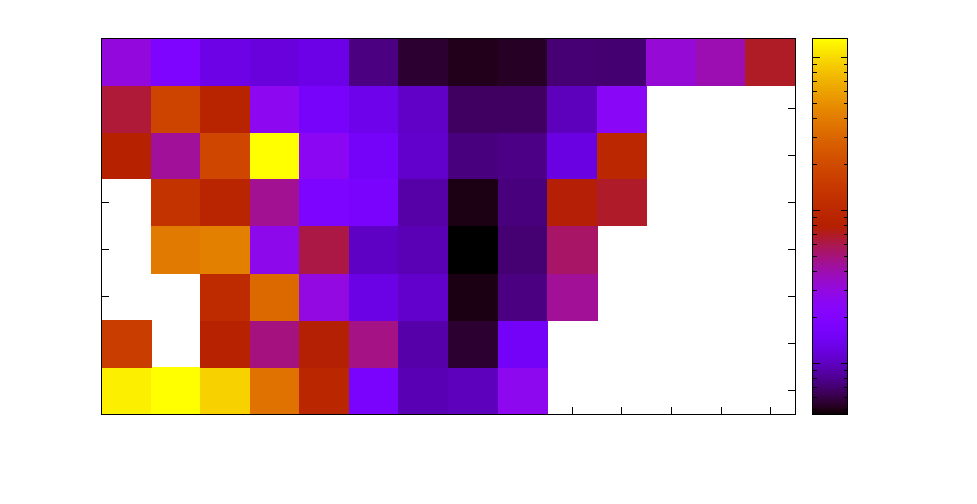
\includegraphics{heat_map}}%
    \gplfronttext
  \end{picture}%
\endgroup
}
			\centering
			\caption{\textit{Heat map of execution time with different values of the parameters $m$ and $\beta$: the darker means the code was faster. White squares means
			convergence was not reached.}}}
			\end{figure}
			\end{frame}
			
			\begin{frame}[fragile]{Profiling with gprof}
				\begin{lstlisting}[language=make]
				profiler: OPTFLAGS=-pg
				profiler: clean $(exec3)
				         ./main_gauss_seidel;\
				         gprof --graph ./main_gauss_seidel\
					               gmon.out > profiling.txt
				\end{lstlisting}
			\end{frame}	
			
			\begin{frame}[fragile]{A C++ program for parameters testing}
				\begin{lstlisting}[basicstyle=\scriptsize, language=C++]
#include <cstdlib>
#include <cstdio>

std::string exec ( const char* cmd ) 
{
	std::array <char, 128> buffer;
	std::string result;
	std::unique_ptr <FILE, decltype(&pclose)> pipe
				(popen(cmd, "r"), pclose);
			
	if (!pipe) {
		throw std::runtime_error("popen() failed!");
	}
	while ( fgets(buffer.data(), buffer.size(), pipe.get() )
						!= nullptr) 
	{
		result += buffer.data();
	}
	return result;
}
				\end{lstlisting}
			\end{frame}
			
			\begin{frame}[fragile]{A C++ program for parameters testing}
						\begin{lstlisting}[basicstyle=\scriptsize, language=C++]
	std::vector <double > parameter {2, 4, ...};
	std::ostringstream tmp;
	tmp << "Parameter = " << parameter[i] << std::flush;
	std::system ( ("sed -i '45s/.*/" + 
	tmp.str() + "/' data.input").c_str() );
	
	double value = stod (exec("./main_gauss_seidel |
	grep 'TIME: Alternating Anderson method' |
			tr -dc '.0-9'"));
			\end{lstlisting}
			\end{frame}
			
			

				
			\begin{frame}[fragile]{Alternating method}
				\begin{itemize}
					\item Consists in alternating a number $p$ of fixed-point iterations to an accelerated step (using Anderson algorithm)
					\item Applied to Jacobi method in \cite{Pratapa}
					\item The standard Anderson method converges in
			about $0.0005 s$
				\end{itemize}

			\begin{figure}
			{\scriptsize
			\resizebox{!}{3.5cm}{
			% GNUPLOT: LaTeX picture with Postscript
\begingroup
  % Encoding inside the plot.  In the header of your document, this encoding
  % should to defined, e.g., by using
  % \usepackage[cp1252,<other encodings>]{inputenc}
  \inputencoding{cp1252}%
  \makeatletter
  \providecommand\color[2][]{%
    \GenericError{(gnuplot) \space\space\space\@spaces}{%
      Package color not loaded in conjunction with
      terminal option `colourtext'%
    }{See the gnuplot documentation for explanation.%
    }{Either use 'blacktext' in gnuplot or load the package
      color.sty in LaTeX.}%
    \renewcommand\color[2][]{}%
  }%
  \providecommand\includegraphics[2][]{%
    \GenericError{(gnuplot) \space\space\space\@spaces}{%
      Package graphicx or graphics not loaded%
    }{See the gnuplot documentation for explanation.%
    }{The gnuplot epslatex terminal needs graphicx.sty or graphics.sty.}%
    \renewcommand\includegraphics[2][]{}%
  }%
  \providecommand\rotatebox[2]{#2}%
  \@ifundefined{ifGPcolor}{%
    \newif\ifGPcolor
    \GPcolorfalse
  }{}%
  \@ifundefined{ifGPblacktext}{%
    \newif\ifGPblacktext
    \GPblacktexttrue
  }{}%
  % define a \g@addto@macro without @ in the name:
  \let\gplgaddtomacro\g@addto@macro
  % define empty templates for all commands taking text:
  \gdef\gplbacktext{}%
  \gdef\gplfronttext{}%
  \makeatother
  \ifGPblacktext
    % no textcolor at all
    \def\colorrgb#1{}%
    \def\colorgray#1{}%
  \else
    % gray or color?
    \ifGPcolor
      \def\colorrgb#1{\color[rgb]{#1}}%
      \def\colorgray#1{\color[gray]{#1}}%
      \expandafter\def\csname LTw\endcsname{\color{white}}%
      \expandafter\def\csname LTb\endcsname{\color{black}}%
      \expandafter\def\csname LTa\endcsname{\color{black}}%
      \expandafter\def\csname LT0\endcsname{\color[rgb]{1,0,0}}%
      \expandafter\def\csname LT1\endcsname{\color[rgb]{0,1,0}}%
      \expandafter\def\csname LT2\endcsname{\color[rgb]{0,0,1}}%
      \expandafter\def\csname LT3\endcsname{\color[rgb]{1,0,1}}%
      \expandafter\def\csname LT4\endcsname{\color[rgb]{0,1,1}}%
      \expandafter\def\csname LT5\endcsname{\color[rgb]{1,1,0}}%
      \expandafter\def\csname LT6\endcsname{\color[rgb]{0,0,0}}%
      \expandafter\def\csname LT7\endcsname{\color[rgb]{1,0.3,0}}%
      \expandafter\def\csname LT8\endcsname{\color[rgb]{0.5,0.5,0.5}}%
    \else
      % gray
      \def\colorrgb#1{\color{black}}%
      \def\colorgray#1{\color[gray]{#1}}%
      \expandafter\def\csname LTw\endcsname{\color{white}}%
      \expandafter\def\csname LTb\endcsname{\color{black}}%
      \expandafter\def\csname LTa\endcsname{\color{black}}%
      \expandafter\def\csname LT0\endcsname{\color{black}}%
      \expandafter\def\csname LT1\endcsname{\color{black}}%
      \expandafter\def\csname LT2\endcsname{\color{black}}%
      \expandafter\def\csname LT3\endcsname{\color{black}}%
      \expandafter\def\csname LT4\endcsname{\color{black}}%
      \expandafter\def\csname LT5\endcsname{\color{black}}%
      \expandafter\def\csname LT6\endcsname{\color{black}}%
      \expandafter\def\csname LT7\endcsname{\color{black}}%
      \expandafter\def\csname LT8\endcsname{\color{black}}%
    \fi
  \fi
    \setlength{\unitlength}{0.0500bp}%
    \ifx\gptboxheight\undefined%
      \newlength{\gptboxheight}%
      \newlength{\gptboxwidth}%
      \newsavebox{\gptboxtext}%
    \fi%
    \setlength{\fboxrule}{0.5pt}%
    \setlength{\fboxsep}{1pt}%
\begin{picture}(5668.00,2834.00)%
    \gplgaddtomacro\gplbacktext{%
      \csname LTb\endcsname%%
      \put(1342,704){\makebox(0,0)[r]{\strut{}0.00005}}%
      \put(1342,1086){\makebox(0,0)[r]{\strut{}0.00010}}%
      \put(1342,1468){\makebox(0,0)[r]{\strut{}0.00015}}%
      \put(1342,1849){\makebox(0,0)[r]{\strut{}0.00020}}%
      \put(1342,2231){\makebox(0,0)[r]{\strut{}0.00025}}%
      \put(1342,2613){\makebox(0,0)[r]{\strut{}0.00030}}%
      \put(1474,484){\makebox(0,0){\strut{}$0$}}%
      \put(1854,484){\makebox(0,0){\strut{}$20$}}%
      \put(2233,484){\makebox(0,0){\strut{}$40$}}%
      \put(2613,484){\makebox(0,0){\strut{}$60$}}%
      \put(2993,484){\makebox(0,0){\strut{}$80$}}%
      \put(3373,484){\makebox(0,0){\strut{}$100$}}%
      \put(3752,484){\makebox(0,0){\strut{}$120$}}%
      \put(4132,484){\makebox(0,0){\strut{}$140$}}%
      \put(4512,484){\makebox(0,0){\strut{}$160$}}%
      \put(4891,484){\makebox(0,0){\strut{}$180$}}%
      \put(5271,484){\makebox(0,0){\strut{}$200$}}%
    }%
    \gplgaddtomacro\gplfronttext{%
      \csname LTb\endcsname%%
      \put(209,1658){\rotatebox{-270}{\makebox(0,0){\strut{}time($s$)}}}%
      \put(3372,154){\makebox(0,0){\strut{}$p$}}%
    }%
    \gplbacktext
    \put(0,0){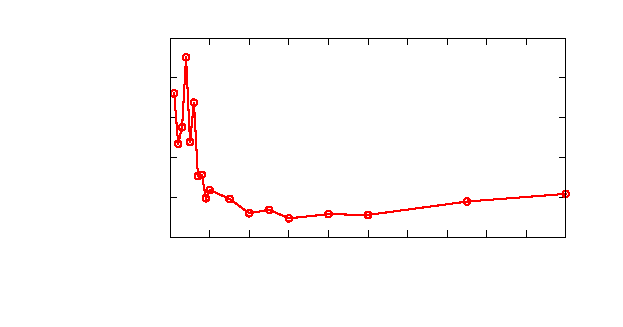
\includegraphics{alternating}}%
    \gplfronttext
  \end{picture}%
\endgroup
}}
			\caption{\textit{Testing different values of parameter $p$ with $\beta=1$ and $m=8$}}
			\centering
			\end{figure}

			\end{frame}
				
				\begin{frame}{Nonlinear problem}
						A thermal radiation term was added, leading to the nonlinear system
			\begin{equation*}
				A u + \sigma I h^2 u^4 = f
			\end{equation*}
			Fixed-point form used:
			\begin{equation*}
				u = (A+ \sigma I h^2 u^3)^{-1} f 
			\end{equation*}
			resulting in the iterative scheme
			\begin{equation*}
				u_{k+1}= (A+ \sigma I h^2 u^3_k)^{-1} f 
			\end{equation*}
			This in turns results in solving at each step the linear system
			\begin{equation*}
				(A+ \sigma I h^2 u^3_k) u_{k+1} = f
			\end{equation*}
			Newton method reads:
			\begin{equation*}
				x_{k+1}= x_k - (A+4 \sigma I h^2 x_k^3)^{-1}(A x_k + \sigma I h^2 x_k^4 - f)
			\end{equation*}
		
				\end{frame}
				
				\begin{frame}{Performances for different solvers}
			\begin{figure}
			{\scriptsize
			% GNUPLOT: LaTeX picture with Postscript
\begingroup
  % Encoding inside the plot.  In the header of your document, this encoding
  % should to defined, e.g., by using
  % \usepackage[cp1252,<other encodings>]{inputenc}
  \inputencoding{cp1252}%
  \makeatletter
  \providecommand\color[2][]{%
    \GenericError{(gnuplot) \space\space\space\@spaces}{%
      Package color not loaded in conjunction with
      terminal option `colourtext'%
    }{See the gnuplot documentation for explanation.%
    }{Either use 'blacktext' in gnuplot or load the package
      color.sty in LaTeX.}%
    \renewcommand\color[2][]{}%
  }%
  \providecommand\includegraphics[2][]{%
    \GenericError{(gnuplot) \space\space\space\@spaces}{%
      Package graphicx or graphics not loaded%
    }{See the gnuplot documentation for explanation.%
    }{The gnuplot epslatex terminal needs graphicx.sty or graphics.sty.}%
    \renewcommand\includegraphics[2][]{}%
  }%
  \providecommand\rotatebox[2]{#2}%
  \@ifundefined{ifGPcolor}{%
    \newif\ifGPcolor
    \GPcolorfalse
  }{}%
  \@ifundefined{ifGPblacktext}{%
    \newif\ifGPblacktext
    \GPblacktexttrue
  }{}%
  % define a \g@addto@macro without @ in the name:
  \let\gplgaddtomacro\g@addto@macro
  % define empty templates for all commands taking text:
  \gdef\gplbacktext{}%
  \gdef\gplfronttext{}%
  \makeatother
  \ifGPblacktext
    % no textcolor at all
    \def\colorrgb#1{}%
    \def\colorgray#1{}%
  \else
    % gray or color?
    \ifGPcolor
      \def\colorrgb#1{\color[rgb]{#1}}%
      \def\colorgray#1{\color[gray]{#1}}%
      \expandafter\def\csname LTw\endcsname{\color{white}}%
      \expandafter\def\csname LTb\endcsname{\color{black}}%
      \expandafter\def\csname LTa\endcsname{\color{black}}%
      \expandafter\def\csname LT0\endcsname{\color[rgb]{1,0,0}}%
      \expandafter\def\csname LT1\endcsname{\color[rgb]{0,1,0}}%
      \expandafter\def\csname LT2\endcsname{\color[rgb]{0,0,1}}%
      \expandafter\def\csname LT3\endcsname{\color[rgb]{1,0,1}}%
      \expandafter\def\csname LT4\endcsname{\color[rgb]{0,1,1}}%
      \expandafter\def\csname LT5\endcsname{\color[rgb]{1,1,0}}%
      \expandafter\def\csname LT6\endcsname{\color[rgb]{0,0,0}}%
      \expandafter\def\csname LT7\endcsname{\color[rgb]{1,0.3,0}}%
      \expandafter\def\csname LT8\endcsname{\color[rgb]{0.5,0.5,0.5}}%
    \else
      % gray
      \def\colorrgb#1{\color{black}}%
      \def\colorgray#1{\color[gray]{#1}}%
      \expandafter\def\csname LTw\endcsname{\color{white}}%
      \expandafter\def\csname LTb\endcsname{\color{black}}%
      \expandafter\def\csname LTa\endcsname{\color{black}}%
      \expandafter\def\csname LT0\endcsname{\color{black}}%
      \expandafter\def\csname LT1\endcsname{\color{black}}%
      \expandafter\def\csname LT2\endcsname{\color{black}}%
      \expandafter\def\csname LT3\endcsname{\color{black}}%
      \expandafter\def\csname LT4\endcsname{\color{black}}%
      \expandafter\def\csname LT5\endcsname{\color{black}}%
      \expandafter\def\csname LT6\endcsname{\color{black}}%
      \expandafter\def\csname LT7\endcsname{\color{black}}%
      \expandafter\def\csname LT8\endcsname{\color{black}}%
    \fi
  \fi
    \setlength{\unitlength}{0.0500bp}%
    \ifx\gptboxheight\undefined%
      \newlength{\gptboxheight}%
      \newlength{\gptboxwidth}%
      \newsavebox{\gptboxtext}%
    \fi%
    \setlength{\fboxrule}{0.5pt}%
    \setlength{\fboxsep}{1pt}%
\begin{picture}(5668.00,2834.00)%
    \gplgaddtomacro\gplbacktext{%
      \csname LTb\endcsname%%
      \put(1210,895){\makebox(0,0)[r]{\strut{}$1\times10^{-8}$}}%
      \put(1210,1277){\makebox(0,0)[r]{\strut{}$1\times10^{-6}$}}%
      \put(1210,1659){\makebox(0,0)[r]{\strut{}$0.0001$}}%
      \put(1210,2040){\makebox(0,0)[r]{\strut{}$0.01$}}%
      \put(1210,2422){\makebox(0,0)[r]{\strut{}$1$}}%
      \put(1342,484){\makebox(0,0){\strut{}$0$}}%
      \put(2128,484){\makebox(0,0){\strut{}$5$}}%
      \put(2914,484){\makebox(0,0){\strut{}$10$}}%
      \put(3699,484){\makebox(0,0){\strut{}$15$}}%
      \put(4485,484){\makebox(0,0){\strut{}$20$}}%
      \put(5271,484){\makebox(0,0){\strut{}$25$}}%
    }%
    \gplgaddtomacro\gplfronttext{%
      \csname LTb\endcsname%%
      \put(209,1658){\rotatebox{-270}{\makebox(0,0){\strut{}Residual}}}%
      \put(3306,154){\makebox(0,0){\strut{}Iteration \#}}%
      \csname LTb\endcsname%%
      \put(4284,2440){\makebox(0,0)[r]{\strut{}Fixed-point iterations}}%
      \csname LTb\endcsname%%
      \put(4284,2220){\makebox(0,0)[r]{\strut{}Newton iterations}}%
      \csname LTb\endcsname%%
      \put(4284,2000){\makebox(0,0)[r]{\strut{}Anderson iterations}}%
      \csname LTb\endcsname%%
      \put(4284,1780){\makebox(0,0)[r]{\strut{}Newton-Anderson}}%
    }%
    \gplbacktext
    \put(0,0){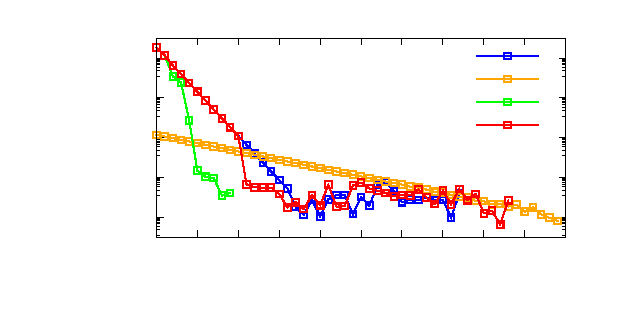
\includegraphics{nonlinear}}%
    \gplfronttext
  \end{picture}%
\endgroup
}
			\centering
			\end{figure}

				\end{frame}
				
				\section{Conclusions}
				\begin{frame}{Conclusions}
					\begin{itemize}
					\item	Anderson algorithm significantly accelerated all the problems considered
					\item The alternating scheme \cite{Pratapa} achieves great speed-ups in the linear case
					\item In the nonlinear problem the performance of Anderson acceleration was almost
						comparable with the one of Newton method.
					\end{itemize}
				\end{frame}
				
				\begin{frame}{References}
					\printbibliography[heading=bibintoc]
				\end{frame}
				
			
			\end{document} 
						